%%%%%%%%%%%%%%%%%%%%%%%%%%%%%%%%%%%%%%%%%
% Beamer Presentation
% LaTeX Template
% Version 1.0 (10/11/12)
%
% This template has been downloaded from:
% http://www.LaTeXTemplates.com
%
% License:
% CC BY-NC-SA 3.0 (http://creativecommons.org/licenses/by-nc-sa/3.0/)
%
%%%%%%%%%%%%%%%%%%%%%%%%%%%%%%%%%%%%%%%%%

%----------------------------------------------------------------------------------------
%	PACKAGES AND THEMES
%----------------------------------------------------------------------------------------

\documentclass{beamer}

\mode<presentation> {

% The Beamer class comes with a number of default slide themes
% which change the colors and layouts of slides. Below this is a list
% of all the themes, uncomment each in turn to see what they look like.

%\usetheme{default}
%\usetheme{AnnArbor}
%\usetheme{Antibes}
%\usetheme{Bergen}
%\usetheme{Berkeley}
%\usetheme{Berlin}
%\usetheme{Boadilla}
%\usetheme{CambridgeUS}
%\usetheme{Copenhagen}
%\usetheme{Darmstadt}
%\usetheme{Dresden}
%\usetheme{Frankfurt}
%\usetheme{Goettingen}
%\usetheme{Hannover}
%\usetheme{Ilmenau}
%\usetheme{JuanLesPins}
%\usetheme{Luebeck}
\usetheme{Madrid}
%\usetheme{Malmoe}
%\usetheme{Marburg}
%\usetheme{Montpellier}
%\usetheme{PaloAlto}
%\usetheme{Pittsburgh}
%\usetheme{Rochester}
%\usetheme{Singapore}
%\usetheme{Szeged}
%\usetheme{Warsaw}

% As well as themes, the Beamer class has a number of color themes
% for any slide theme. Uncomment each of these in turn to see how it
% changes the colors of your current slide theme.

%\usecolortheme{albatross}
%\usecolortheme{beaver}
%\usecolortheme{beetle}
%\usecolortheme{crane}
%\usecolortheme{dolphin}
%\usecolortheme{dove}
%\usecolortheme{fly}
%\usecolortheme{lily}
%\usecolortheme{orchid}
%\usecolortheme{rose}
%\usecolortheme{seagull}
%\usecolortheme{seahorse}
%\usecolortheme{whale}
%\usecolortheme{wolverine}
%\usecolortheme{default}

\usefonttheme{default}  % or try serif, structurebold, ...

%\setbeamertemplate{footline} % To remove the footer line in all slides uncomment this line
%line in all slides with a simple slide count uncomment this line
%\setbeamertemplate{blocks}[rounded][shadow=true]
%\setbeamertemplate{footline}[page number] % To replace the footer
%\setbeamertemplate{caption}[numbered]
%\setbeamertemplate{background canvas}[vertical shading][bottom=white,top=structure.fg!25]
%\setbeamertemplate{sidebar canvas left}[horizontal shading][left=white!40!black,right=black]
%\setbeamertemplate{navigation symbols}{} % To remove the navigation
%symbols from the bottom of all slides uncomment this line


}



%\usepackage{graphicx} % Allows including images
%\usepackage{booktabs} % Allows the use of \toprule, \midrule and
                      % \bottomrule in tables
\usepackage{graphicx,caption}
\usepackage[brazil]{babel} % este é para o texto

%----------------------------------------------------------------------------------------
%	TITLE PAGE
%----------------------------------------------------------------------------------------

\title[Proveni\^encia de dados]{Proveni\^encia de dados em workflow de Bioinform\'atica com PROV-DM e armazenamento em banco de dados baseado em grafo} % The short title appears at the bottom of every slide, the full title is only on the title page

\author{Rodrigo Pinheiro} % Your name
%Exame de Qualifica\c{c}\~ao de Mestrado Programa de P\'os-Graduação em Inform\'atica
\institute[UnB] % Your institution as it will appear on the bottom of every slide, may be shorthand to save space
{
Universidade de Bras\'ilia \\ % Your institution for the title page
\medskip
Exame de Qualifica\c{c}\~ao de Mestrado Programa de P\'os-Gradua\c{c}\~ao em
Inform\'atica
Orientador(a): Maristela Terto de Holanda
}
\date{\today} % Date, can be changed to a custom date

\begin{document}

\begin{frame}
\titlepage % Print the title page as the first slide
\end{frame}

\begin{frame}
\frametitle{Agenda} % Table of contents slide, comment this block out to remove it
\tableofcontents % Throughout your presentation, if you choose to use \section{} and \subsection{} commands, these will automatically be printed on this slide as an overview of your presentation
\end{frame}

%----------------------------------------------------------------------------------------
%	PRESENTATION SLIDES
%----------------------------------------------------------------------------------------

%------------------------------------------------
\section{Contextualiza\c{c}\~ao} % Sections can be created in order to organize your presentation into discrete blocks, all sections and subsections are automatically printed in the table of contents as an overview of the talk
%------------------------------------------------

%\subsection{Workflow na Bioinform\'atica} % A subsection can be created just before a set of slides with a common theme to further break down your presentation into chunks

\begin{frame}
\frametitle{\textit{Workflow} na Bioinform\'atica}
\begin{figure}
\centering
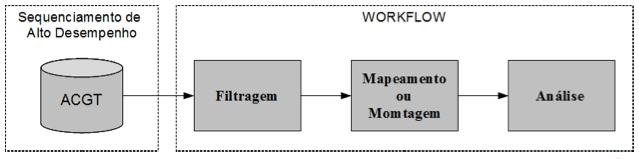
\includegraphics[width=200pt]{images/workflowBioinformatica.png}
\caption{Exemplo de workflow para projetos genoma e transcritoma.}
\label{fig:entidadeprovdm}
\end{figure}
\begin{itemize}
\item A execu\c{c}\~ao de um \textit{workflow} pode levar dias ou semanas;
\item \'E necess\'ario re-executar um experimento e valid\'a-lo;
\end{itemize}
%\begin{itemize}
%\item Filtragem: filtra as \textit{reads} com qualidade inferior e
 % pode detectar outros contaminantes ou erros labotoriais.
%\item Mapeamento ou montagem: 
%   \begin{itemize}
%     \item Mapeamento: a fase de mapeamento tenta localizar, em
%  um genoma de refer\^encia, as \textit{reads} filtradas. 
%      \item Montagem: quando n\~ao \'e
%  conhecido o genoma de referência pode-se alinhar as \textit{reads}
%  entre elas gerando sequ\^encias maiores chamadas
%  \textit{contigs}. 
%  \end{itemize}
%\item Análise: Nesta fase tem-se grandes por\c{c}\~oes do DNA ou RNA mapeadas que podem ser analisadas por diferentes processos dependendo do objetivo do experimento.
%\end{itemize}
\end{frame}

%------------------------------------------------
%\subsection{Proveni\^encia de dados}

\begin{frame}
\frametitle{O que \'e proveni\^encia de dados?}
\begin{block}{Defini\c{c}\~ao}
O termo Proveni\^encia de dados diz respeito \`a origem ou
proced\^encia dos dados. A proveni\^encia tamb\'em pode se referir \`a
auditoria, triagem, linhagem e origem do dado \cite{p2}.
\end{block}
\begin{itemize}
\item Segundo \cite{p3}, pode-se dividir o n\'ivel em que \'e feita a
  captura conforme segue:
\begin{itemize}
\item \textit{Workflow}: envolve a descri\c{c}\~ao da execu\c{c}\~ao de um
  processo;
\item Atividade: pode ocorrer de duas formas. Na primeira, cada
  processo executado \'e alterado para capturar os dados de
  proveni\^encia. Na segunda, podem ser criados programas
  espec\'ificos para monitorar a execu\c{c}\~ao de um determinado
  processo e capturar os dados de proveni\^encia;
\item Sistema Operacional: utiliza os dados fornecidos pelo pr\'oprio sistema operacional como insumo para a proveni\^encia.
\end{itemize}
\end{itemize}

\end{frame}

%------------------------------------------------
%\subsubsection{Modelos de Proveni\^encia}

%------------------------------------------------
\begin{frame}
\frametitle{Modelos de Proveni\^encia}
\begin{block}{Defini\c{c}\~ao}
Tem como principal objetivo fornecer uma estrutura para que os dados
de proveni\^encia possam ser armazenados e recuperados, mantendo seu significado e potencializando os seus benef\'icios. 
\end{block}
\begin{itemize}
\item Modelo W7: objetiva descrever as propriedades de um objeto de
  car\'ater geral;
\item \textit{Provenance Vocabulary}: volta a sua aten\c{c}\~ao para o
  problema da proveni\^encia de dados publicados na \textit{web};
\item \textit{Provenir Ontology}: foi desenvolvido para ser um modelo
  de proveni\^encia de dados gen\'erico;
\item OPM (\textit{Open Provenance Model}): procura demonstrar a
  rela\c{c}\~ao causal entre eventos que afetam objetos (digitais ou
  n\~ao) e descreve essa rela\c{c}\~ao atrav\'es de um grafo
  ac\'iclico direcionado.
\end{itemize}
\end{frame}

%------------------------------------------------
%\subsubsection{PROV-DM}

%------------------------------------------------
\begin{frame}
\frametitle{PROV-DM}
\begin{itemize}
\item Teve a sua primeira vers\~ao desenvolvida em outubro de 2011,
  tornando-se uma recomenda\c{c}\~ao do W3C em Abril de 2013;
\item Tem como principal fun\c{c}\~ao descrever as pessoas, entidades
  e atividades envolvidas na produ\c{c}\~ao de uma pe\c{c}a de dado ou de
  um objeto qualquer;
\item Cria as condi\c{c}\~oes para que a proveni\^encia seja
  demonstrada e trocada entre diferentes sistemas;
\item Demonstra a proveni\^encia de qualquer objeto (real ou
  imagin\'ario) atrav\'es de um grafo direcionado;
\item S\'imbolo para representar grandes conjuntos de dados;
\end{itemize}
\end{frame}

%------------------------------------------------
\begin{frame}
\frametitle{Componentes}
\begin{figure}
\centering
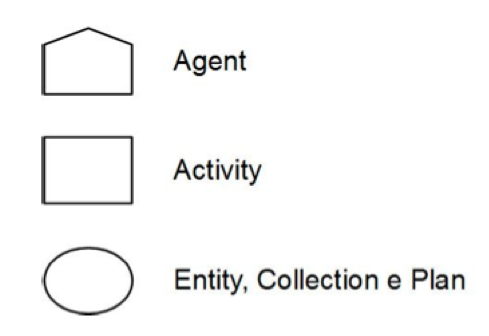
\includegraphics[width=150pt]{images/componentesprovdm.png}
\caption{Representa\c{c}\~ao gr\'afica dos diferentes tipos no modelo
  PROV-DM. \cite{p5}}
\label{fig:entidadeprovdm}
\end{figure}
\begin{itemize}
\item Entidades: podem representar qualquer objeto (real ou
  imagin\'ario);
\item Atividades: \'e algo que ocorre ao longo de um per\'iodo de
  tempo e atua sobre ou com entidades;
\end{itemize}
\end{frame}

%------------------------------------------------
\begin{frame}
\frametitle{Componentes}
\begin{itemize}
\item Agente: s\~ao entidades que influenciam,
  direta ou indiretamente, a execu\c{c}\~ao das atividades;
\item Cole\c{c}\~oes: s\~ao entidades que possuem membros, os quais
  s\~ao tamb\'em entidades;
\item Anota\c{c}\~oes: fornece mecanismos para inclus\~ao de
  anota\c{c}\~oes para os elementos do modelo;
\item Plano: representa um conjunto de a\c{c}\~oes ou passos que um Agente
  deve seguir para chegar a um determinado objetivo;
\item Conta: representa um conjunto de informa\c{c}\~oes (tipos e
  rela\c{c}\~oes) que comp\~oe um grafo de proveni\^encia.
\end{itemize}
\end{frame}

%------------------------------------------------
\begin{frame}
\frametitle{Rela\c{c}\~oes}
\begin{figure}
\centering
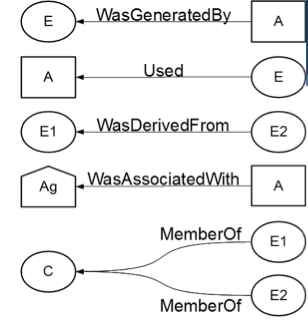
\includegraphics[width=150pt]{images/relacoesprovdm.png}
\caption{Representa\c{c}\~ao gr\'afica das diferentes rela\c{c}\~oes no modelo
  PROV-DM. \cite{p5}}
\label{fig:entidadeprovdm}
\end{figure}
\end{frame}

%------------------------------------------------

\begin{frame}
\frametitle{Rela\c{c}\~oes}
\begin{itemize}
\item \textit{used}: indica que uma Entidade foi usada por uma Atividade;
\item \textit{wasGeneratedBy}: indica que uma Entidade foi gerada por uma Atividade;
\item \textit{wasAttributedTo}: atribui algum tipo de responsabilidade a um Agente sobre uma Entidade;
\item \textit{wasAssociatedWith}: atribui algum tipo de responsabilidade a um
  Agente sobre uma Atividade;
\item \textit{wasDerivedFrom}: indica, de forma geral, que uma Entidade
  (original) foi usada, direta ou indiretamente, na gera\c{c}\~ao de
  outra Entidade (derivada);
\item \textit{memberOf} : indica que uma determinada Entidade \'e membro de uma Cole\c{c}\~ao.
\end{itemize}
\end{frame}

%------------------------------------------------
\begin{frame}
\frametitle{Resti\c{c}\~oes}
\begin{itemize}
\item Restri\c{c}\~oes de Atividade: restri\c{c}\~oes relacionadas \`a
  execu\c{c}\~ao das Atividades.
\begin{itemize}
\item In\'icio/Fim: o in\'icio da execu\c{c}\~ao de uma Atividade deve
  preceder o seu fim;
\item Uso: o uso de uma Entidade por uma Atividade deve ocorrer entre o in\'icio e o
fim da sua execu\c{c}\~ao;
\item Gera\c{c}\~ao: a gera\c{c}\~ao de uma Entidade por uma Atividade deve ocorrer entre o in\'icio e o fim da sua execu\c{c}\~ao.
\end{itemize}
\item Restri\c{c}\~oes de Agente - restri\c{c}\~ao relacionada ao
  ciclo de vida de um Agente.
\begin{itemize}
\item Associa\c{c}\~ao: a associa\c{c}\~ao entre um Agente e uma Atividade deve ocorrer entre
o in\'icio e o fim da execu\c{c}\~ao desta Atividade.
\end{itemize}
\end{itemize}
\end{frame}

%------------------------------------------------
\begin{frame}
\frametitle{Resti\c{c}\~oes}

\begin{itemize}
\item Restri\c{c}\~oes de Entidade - restri\c{c}\~oes relacionadas ao
  ciclo de vida de uma Entidade.
\begin{itemize}
\item Gera\c{c}\~ao/Uso: a gera\c{c}\~ao de uma Entidade deve preceder
  o seu uso;
\item Deriva\c{c}\~ao/Uso/Gera\c{c}\~ao: para os casos em que existe
  uma deriva\c{c}\~ao entre duas Entidades, por exemplo E2 \'e
  derivado de E1, e o uso de E1 \'e conhecido, ent\~ao o uso de E1
  deve preceder a gera\c{c}\~ao de E2;
\item Deriva\c{c}\~ao/Gera\c{c}\~ao/Gera\c{c}\~ao: para os casos em
  que existe uma deriva\c{c}\~ao entre duas Entidades, por exemplo E2
  \'e derivado de E1, e o uso de E1 n\~ao \'e conhecido, ent\~ao a
  gera\c{c}\~ao de E1 deve preceder a gera\c{c}\~ao de E2.
\end{itemize}
\end{itemize}
\end{frame}

%------------------------------------------------
\begin{frame}
\frametitle{Por que PROV-DM em projetos de Bioinform\'atica?}
De acordo com \cite{p10} as raz\~oes de usar o modelo PROV-DM s\~ao:
\begin{itemize}
\item A aplica\c{c}\~ao do modelo PROV-DM em projetos de
  Bioinform\'atica se mostrou simples e direta;
\item Os componentes do modelo, tais como o agente, atividade e
  cole\c{c}\~ao, representam elementos presentes em grande parte dos
  experimentos executados em projetos de Bioinfom\'atica;
\item As rela\c{c}\~oes, por sua vez, demonstram de forma objetiva as
  depend\^encias entre cada elemento no grafo;
\item Utiliza\c{c}\~ao das regras e do tipo de deriva\c{c}\~ao permitem maior grau de especificidade quando necess\'ario.
\end{itemize}
\end{frame}

%\subsection{Armazenamento de dados na nuvem baseado em NoSQL}

%------------------------------------------------
\begin{frame}
\frametitle{Ambiente de computa\c{c}\~ao em nuvem}
\begin{itemize}
\item O ambiente de computa\c{c}\~ao em nuvem tem se tornado atraente
  para a execu\c{c}\~ao de experimentos cient\'ificos devido:
\begin{itemize}
\item Escabilidade;
\item Interoperabilidade;
\item Id\'eia de recursos infinitos.
\end{itemize}
\end{itemize}
\begin{block}{}
Por\'em, informa\c{c}\~oes como par\^ametros de entrada e sa\'ida, tempo de execu\c{c}\~ao,
m\'etodos invocados e processos iniciados e finalizados s\~ao
importantes na execu\c{c}\~ao de experimentos cient\'ificos, porque h\'a a necessidade de validar o experimento e reproduz\'i-lo.
\end{block}
\end{frame}

%------------------------------------------------
\begin{frame}
\frametitle{Bancos de dados no ambiente de computa\c{c}\~ao em
  nuvem}
\begin{block}{}
Para um ambiente heterog\^eneo, distribu\'ido e de alta disponibilidade como o de computa\c{c}\~ao em nuvens, os bancos relacionais n\~ao apresentam um bom desempenho, surgindo os bancos de dados \textit{NoSQL}.
\end{block}
\begin{itemize}
\item \textit{NoSQL}
\begin{itemize}
\item Gerenciam grades volumes de dados;
\item Em geral, fornecem garantias de consist\^encia fraca, estruturas e interfaces simples.
\end{itemize}
\end{itemize}
\begin{block}{}
Como um tipo de bancos de dados \textit{NoSQL}, se destacam os bancos de dados de grafos que permitem o armazenamento de entidades e tamb\'em relacionamentos entre essas entidades.
\end{block}
\end{frame}

%------------------------------------------------
\begin{frame}
\frametitle{Classifica\c{c}\~ao dos bancos \textit{NoSQL}}
\begin{itemize}
\item Os bancos \textit{NoSQL} podem ser classificados em quatro classes gerais
  \cite{p6}:
\begin{itemize}
\item Chave/Valor: os dados s\~ao armazenados como pares chave-valor
  que s\~ao indexados para recupera\c{c}\~ao por chaves. Os mais
  populares s\~ao o \textit{Riak}, \textit{Redis}, \textit{Memcached}, \textit{Berkeley DB}, \textit{Amazon
  DynamoDB}, \textit{Porject Voldemort} e \textit{HamsterDB};
\item Orientado a coluna: armazena os dados em linhas com colunas
  associadas, fazendo uso de uma chave de linha. Exemplos s\~ao o
  \textit{BigTable}, \textit{Cassandra} e \textit{HBase};
\item Armazenamento baseado em documentos: os dados s\~ao armazenados
  e organizados como uma cole\c{c}\~ao de documentos. Exemplos s\~ao o
  \textit{MongoDB}, \textit{Apache CouchDB} e \textit{RavenDB};
\item Bancos de dados de grafos: permitem armazenar entidades e
  tamb\'em relacionamentos entre essas entidades. Exemplos: \textit{Neo4J},
  \textit{Infinite Graph}, \textit{OrientDB} e \textit{FlockDB}.
\end{itemize}
\end{itemize}
\end{frame}

%------------------------------------------------
%\subsection{Modelo de dados de grafo}
%------------------------------------------------

\begin{frame}
\frametitle{Modelo de dados de grafo}
\begin{block}{Defini\c{c}\~ao}
O modelo de dados de grafo \'e uma estrutura na qual o esquema e/ou
inst\^ancias s\~ao modeladas como um grafo dirigido, possivelmente
rotulado, ou generaliza\c{c}\~oes da estrutura de dados do grafo, onde
a manipula\c{c}\~ao de dados \'e expressa por opera\c{c}\~oes orientadadas
para o grafo e construtores de tipos, e restri\c{c}\~oes de
integridade que podem ser definidas sobre a estrutura do grafo. \cite{p7}
\end{block}
Tem-se em \cite{p7} as principais vantagens de se usar esse tipo de
modelo:
\begin{itemize}
\item Permite uma modelagem mais natural dos dados porque as
  estruturas de grafos s\~ao vis\'iveis para o usu\'ario;
\item Permite expressar as consultas em um n\'ivel maior de
  abstra\c{c}\~ao;
\item Permite a implementa\c{c}\~ao de algoritmos eficientes para
  realizar espec\'ificas opera\c{c}\~oes.
\end{itemize}
\end{frame}

%------------------------------------------------

\begin{frame}
\frametitle{Componentes}
\begin{itemize}
\item Entidade/Objeto: representa algo que existe como uma unidade
  simples e completa;
\item Rela\c{c}\~ao: \'e uma propriedade ou predicado que estabelece
  uma conex\~ao entre duas ou mais entidades;
\item Atributos: informa\c{c}\~oes associadas a n\'os e arestas;
\item Direcionamento: dependendo do problemas a rela\c{c}\~ao entre
  dois n\'os pode ser sim\'etrica ou n\~ao. Se a rela\c{c}\~ao \'e
  sim\'etrica, as duas pontas da aresta s\~ao diferentes, mas
  indistingu\'iveis, ou seja, n\~ao h\'a ponta inicial nem ponta
  final. Se a rela\c{c}\~ao n\~ao \'e sim\'etrica, \'e poss\'ivel
  diferenciar as duas pontas da aresta;
\item N\'os e arestas rotuladas: em algumas aplica\c{c}\~oes, \'e
  poss\'ivel diferenciar r\'otulos (ou tipos) de n\'os e arestas.
\end{itemize}
\end{frame}

%------------------------------------------------

\begin{frame}
\frametitle{Opera\c{c}\~oes}
\begin{itemize}
\item Travessias: s\~ao opera\c{c}\~oes que se iniciam de um \'unico
  n\'o e explora recursivamente os vizinhos at\'e que uma
  condi\c{c}\~ao seja alcan\c{c}ada, tais como a profundidade ou
  visitar um n\'o de destino;
\item An\'alise Gr\'afica: basicamente inclui o estudo da topologia de
  grafos para analisar a sua complexidade e para caracterizar objetos
  do grafo;
\item Transforma\c{c}\~ao: compreende as opera\c{c}\~oes que alteram o
  banco de dados de grafo. Cargas de um grafo, adicionar/remover n\'os
  ou arestas dos grafos, criar novos tipos de n\'os/arestas/ atributos
  ou modificar o valor de um atributo;
\item Atributos: bancos de dados n\~ao s\'o tem que gerir a
  informa\c{c}\~ao estrutural do grafo, mas tamb\'em dos dados
  associados \`as entidades do grafo;
\item Resultado: grafos, agregados e conjuntos. 
\end{itemize}
\end{frame}

%------------------------------------------------

\begin{frame}
\frametitle{Banco de dados relacional versus Banco de dados de grafo}
De acordo com \cite{p8}:
\begin{table}[h]
 \caption{\ Compara\c{c}\~ao MySQL versus Neo4J. Requisitos objetivos.}
\begin{tabular}{|c|c|c|c|}
\hline
\multicolumn{1}{|l}{Banco de dados} & \multicolumn{1}{|l}{\begin{tabular}[c]{@{}c@{}}Consultas \\ estruturais\end{tabular}} & \multicolumn{1}{|l}{\begin{tabular}[c]{@{}c@{}}Buscas \\ textuais\end{tabular}} & \multicolumn{1}{|l|}{\begin{tabular}[c]{@{}c@{}}Consultas de \\ contagem num\'erica\end{tabular}} \\ \hline
MySQL                               &                                                                                       &                                                                                 & x                                                                                               \\ \hline
Neo4J                               & x                                                                                     & x                                                                               &                                                                                                 \\ \hline
\end{tabular}
\end{table}

\begin{table}[h]
\caption{\ Compara\c{c}\~ao MySQL versus Neo4J. Requisitos subjetivos.}
\begin{tabular}{|c|c|c|c|c|}
\hline
\multicolumn{1}{|l}{Banco de dados} & \multicolumn{1}{|l}{\begin{tabular}[c]{@{}c@{}}Maturidade\end{tabular}} & \multicolumn{1}{|l}{Flexibilidade} & \multicolumn{1}{|l|}{Suporte} & Seguran\c{c}a \\ \hline
MySQL                               & x                                                                                  &                                    & x                             & x        \\ \hline
Neo4J                               &                                                                                    & x                                  &                               &          \\ \hline
\end{tabular}
\end{table}
\end{frame}

%------------------------------------------------

\begin{frame}
\frametitle{Banco de dados relacional versus Banco de dados de grafo}
Em \textit{Neo4J In Action}, \cite{p9} executou um
experimento comparando um banco de dados relacional com o banco de
dados de grafos Neo4J. Como resultado tem-se a tabela abaixo:
\begin{table}[!h]
\centering
  \large
  \setlength{\arrayrulewidth}{2\arrayrulewidth}
  \setlength{\belowcaptionskip}{10pt}
  \caption{\ Compara\c{c}\~ao MySQL versus Neo4J. \cite{p9}}
  \scalebox{0.8}{
\begin{tabular}{|c|c|c|c|}
\hline
\multicolumn{1}{|l}{Profundidade} & 
\multicolumn{1}{|l}{\begin{tabular}[c]{@{}c@{}}Tempo de execu\c{c}\~ao\\  no MySQL (s)\end{tabular}} &
\multicolumn{1}{|l}{\begin{tabular}[c]{@{}c@{}}Tempo de execu\c{c}\~ao\\  no Neo4J (s)\end{tabular}} &
\multicolumn{1}{|l|}{Registros retornados} \\ \hline
2                                 & 0.016                                                                                          & 0.01                                                & 2.500                                      \\ \hline
3                                 & 30.267                                                                                         & 0.168                                               & 110.000                                    \\ \hline
4                                 & 1543.505                                                                                       & 1.359                                               & 600.000                                    \\ \hline
5                                 & ---                                                                                            & 2.132                                               & 800.000                                    \\ \hline
\end{tabular}}
\label{tab:mysqlneo4j}
\end{table}
\end{frame}

%------------------------------------------------
%\subsection{Proposta}
%------------------------------------------------
\begin{frame}
\frametitle{Contextualiza\c{c}\~ao da Proposta}
\begin{block}{}
Como apresentado em \cite{p10}, o modelo PROV-DM pode ser
aplicado em workflow de Bioinform\'atica onde atrav\'es de um grafo
\'e poss\'ivel facilmente representar a proveni\^encia em um
experimento da Bioinform\'atica salvando os dados em arquivos XML.
\end{block}
\begin{block}{}
Em \cite{p18} \'e proposto a captura autom\'atica de
dados e o armazenamento em um esquema relacional baseado no modelo
PROV-DM.
\end{block}
\begin{block}{}
Como o PROV-DM \'e um modelo baseado em grafo, onde toda proveni\^encia
pode ser representada atrav\'es de n\'os e arestas.
\end{block}
\begin{block}{}
A execu\c{c}\~ao do workflow em um ambiente de computa\c{c}\~ao em
nuvem \'e uma realidade em v\'arios experimentos na Bioinform\'atica.
\end{block}
\end{frame}

%------------------------------------------------

\begin{frame}
\frametitle{Proposta}
\begin{block}{}
Realizar a proveni\^encia de dados em projetos de Bioinform\'atica
utilizando um modelo de proveni\^encia PROV-DM e armazenando os dados em bancos de dados de grafos no ambiente de computa\c{c}\~ao em nuvem. 
\end{block}
\begin{itemize}
\item Objetivos espec\'ificos
\begin{itemize}
\item Definir uma arquitetura de proveni\^encia de dados para um ambiente de computa\c{c}\~ao em nuvem em projetos de Bioinform\'atica, utilizando bancos de dados de grafos;
\item Implementar a arquitetura proposta;
\item Realizar estudo de caso com workflows cient\'ificos reais da
  Bioinform\'atica;
\item Avaliar os resultados obtidos. 
\end{itemize}
\end{itemize}
\end{frame}

%------------------------------------------------
\section{Fundamenta\c{c}\~ao Te\'orica}
%------------------------------------------------

%------------------------------------------------

\begin{frame}
\frametitle{Fundamenta\c{c}\~ao Te\'orica}
\begin{itemize}
\item \textit{Provenance for the cloud}. \cite{p11}: defende a proveni\^encia como primeiro conjunto de dados a ser
  salvo no ambiente de computa\c{c}\~ao em nuvem;
\item Captura de Metadados de Proveni\^encia para Workflows
  Cient\'ificos em Nuvens Computacionas.  \cite{p12}: apoia a coleta de metadados de proveni\^encia em experimentos
  cient\'ificos para o ambiente de computa\c{c}\~ao em nuvem;
\item Reprodu\c{c}\~ao de Experimentos Cient\'ificos Usando
  Nuvens. \cite{p13}: visa a reprodu\c{c}\~ao do ambiente onde o
  experimento computacional foi originalmente executado;
\item \textit{Capturing and querying workflow runtime provenance with
    prov: A practical approach.} \cite{p14}: prop\~oe uma
  solu\c{c}\~ao para monitorar o experimento durante a sua
  execu\c{c}\~ao, usando dados de proveni\^encia;
\end{itemize}
\end{frame}

%------------------------------------------------

\begin{frame}
\frametitle{Fundamenta\c{c}\~ao Te\'orica}
\begin{itemize}
\item \textit{Performance analysis of data filtering in scientific
    workflows.} \cite{p15}: prop\~oe melhorar a performance de workflows cient\'ificos,
  reduzindo os dados a serem processados pelas atividades atrav\'es de
  dados de proveni\^encia;
\item \textit{Provenance in bioinformatics workflows.} \cite{p10}: prop\~oe uso de proveni\^encia de dados com base no modelo
  PROV-DM para fluxos de trabalho de projetos genoma;
\item \textit{Achieving reproducibility by combining provenance with
    service and workflow versioning.} \cite{p16}: trata de como um sistema de armazenamento de proveni\^encia \'e
  usado pela plataforma de computa\c{c}\~ao em nuvem e-Science
  Central;
\item \textit{Prob: A tool for tracking provenance and reproducibility
    of big data experiments.} \cite{p17}: usa uma ferramenta de captura de dados de proveni\^encia para
  alcan\c{c}ar a reprodu\c{c}\~ao de experimentos cient\'ificos
  envolvidos com \textit{workflow} de \textit{big data}, o PROB;
\end{itemize}
\end{frame}

%------------------------------------------------
\begin{frame}
\frametitle{Resumo Referencial Te\'orico}
\begin{table}[!h]
  \centering
  \large
  \setlength{\arrayrulewidth}{1\arrayrulewidth}
  \setlength{\belowcaptionskip}{5pt}
  \caption{\ Resumo referencial te\'orico.}
  \scalebox{0.7}{
  \begin{tabular}{|p{4cm}|p{2.5cm}|p{3.5cm}|p{4cm}|}
     \hline
     \hline
     \textbf{Proposta} & \textbf{Modelo de proveni\^encia} & \textbf{Ambiente de execu\c{c}\~ao} & \textbf{Sistema de armazenamento} \\
     \hline
     [Muniswamy-Reddy et al, 2010] & --- & Computa\c{c}\~ao  em nuvem &  \textit{Storage} \\
     \hline
     \cite{p12} & OPM & Computa\c{c}\~ao em nuvem &  Banco de dados relacional \\
     \hline
     [de Oliveira et al., 2012] & PROV-DM & \textit{Dekstop} &  Banco de dados relacional \\
     \hline
     \cite{p14} & PROV-DM & \textit{Dekstop} e Computa\c{c}\~ao em nuvem &  Banco de dados relacional \\
     \hline
     [Goncalves et al., 2013] & --- & Computa\c{c}\~ao em nuvem &  Banco de dados relacional \\
     \hline
     [de Paula et al., 2013] & PROV-DM & \textit{Dekstop} &  Arquivo \textit{XML} \\
     \hline
     [Woodman et al., 2011] & OPM & Computa\c{c}\~ao em nuvem &  Banco de dados de
     grafo\\
     \hline
     [Korolev and Joshi, 2014] & PROV-DM & Computa\c{c}\~ao em nuvem &  Sistema de
     versionamento \textit{GitHub} \\
     \hline
  \end{tabular}}
\label{tab:resumoreferencial}
\end{table}
\end{frame}

%------------------------------------------------
\section{Arquitetura Proposta}
%------------------------------------------------

\begin{frame}
\frametitle{Arquitetura Proposta}
\begin{itemize}
\item Existem na literatura trabalhos usando os modelos de
  proveni\^encia OPM e PROV-DM;
\item Armazenamento dos dados de proveni\^encia em bancos de dados de
  grafos; 
\item Proveni\^encia de dados para processos executados em um ambiente
  de computa\c{c}\~ao em nuvem.
\end{itemize}
\begin{block}{}
Por\'em n\~ao tratam de um modelo de dados para proveni\^encia de
workflow de Bioinform\'atica usando bancos de dados de grafos para
armazenar os dados do modelo PROV-DM com execu\c{c}\~ao em um ambiente
de computa\c{c}\~ao em nuvem.
\end{block}
\end{frame}

%------------------------------------------------

\begin{frame}
\frametitle{Modelo de dados em bancos de dados de grafo}
\begin{itemize}
\item Os dois tipos b\'asicos do modelo PROV-DM, atividade e entidade
  ser\~ao representados como n\'os no banco de dados de grafo, e
  ser\~ao diferenciados pela propriedade Tipo.
\item J\'a as rela\c{c}\~oes ser\~ao representadas pelas arestas,
  sendo diferenciadas tamb\'em por uma propriedade Tipo. 
\end{itemize}
\begin{figure}[h!]
\centering
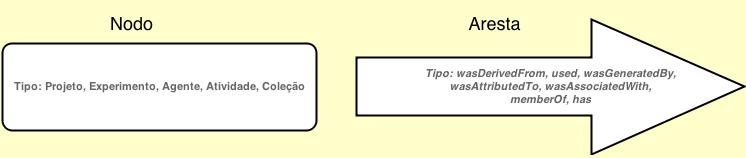
\includegraphics[width=350pt]{images/NodoEAresta.jpg}
\caption{Mapeamento dos tipos e rela\c{c}\~oes para o modelo de dados baseado em grafo.}
\label{fig:nodoaresta}
\end{figure}
\end{frame}

%------------------------------------------------

\begin{frame}
\frametitle{Arquitetura Proposta}
\begin{figure}[h!]
\centering
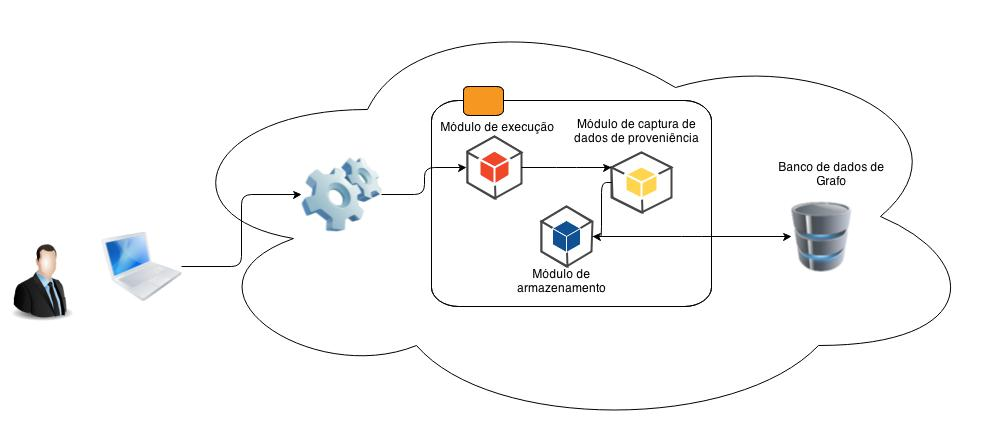
\includegraphics[width=350pt]{images/ArquiteturaPropostaII.jpg}
\caption{Arquitetura Proposta.}
\label{fig:arquitetura}
\end{figure}
\end{frame}

%------------------------------------------------

\begin{frame}
\frametitle{Arquitetura Proposta}
\begin{itemize}
\item Uma interface web simples e amig\'avel para o usu\'ario,
  permitindo-o criar projetos, experimentos e atividades. Os dados
  informados pelo usu\'ario ser\~ao enviados para a nuvem para serem
  processados;
\item M\'odulo de execu\c{c}\~ao: respons\'avel por executar os
  comandos ou programas recebidos do usu\'ario;
\item M\'odulo de captura de dados de proveni\^encia: respons\'avel
  por receber os dados informados pelo usu\'ario, interpret\'a-los e
  realizar a captura da proveni\^encia de forma autom\'atica;
\item M\'odulo de armazenamento: ser\'a respons\'avel pela
  comunica\c{c}\~ao com o banco de dados de grafo e prover uma
  interface de acesso;
\item Banco de dados de grafo: respons\'avel pelo armazenamento dos
  dados na forma de grafo.
\end{itemize}
\end{frame}

%------------------------------------------------
\section{Metodologia e Cronograma}
%------------------------------------------------

\begin{frame}
\frametitle{Metodologia}
\begin{itemize}
\item Primeira fase: estudo e an\'alise;
\item Segunda fase: especifica\c{c}\~ao da arquitetura;
\item Terceira fase: implementa\c{c}\~ao;
\item Quarta fase: testes;
\item Quinta fase: avalia\c{c}\~ao e corre\c{c}\~ao;
\item Sexta fase: publica\c{c}\~ao e defesa da disserta\c{c}\~ao.
\end{itemize}
\end{frame}

%------------------------------------------------

\begin{frame}
\frametitle{Cronograma}
\begin{block}{}
Foi realizada a publica\c{c}\~ao do artigo \cite{p18} na confer\^encia
\textit{The IEEE International Conference on Bioinformatics and Biomedicine (BIBM)} de 2013, que prop\~oe a
  captura autom\'atica de dados de proveni\^encia e o armazenamento em
  um esquema relacional baseado no modelo PROV-DM.
\end{block}
\begin{table}[!h]
  \centering
  \large
  \setlength{\arrayrulewidth}{2\arrayrulewidth}
  \setlength{\belowcaptionskip}{3pt}
  \caption{\ Cronograma de atividades.}
  \scalebox{0.8}{
  \begin{tabular}{|c|c|c|c|c|c|c|}
     \hline
%	\multicolumn{1}{|c|}{""} & \multicolumn{6}{|c|}{\textbf{Ano 2013}}\\ 
     \hline
     \textbf{Etapa} & \textbf{2013/1} & \textbf{2013/2} & \textbf{2014/1} & \textbf{2014/2} \\
     \hline
     1 & X & X & X & \\    
     \hline
     2 &  & X & X &   \\    
     \hline
     3 & & & X & \\
     \hline
     4 &  & & X & X \\
     \hline
     5 & & &  & X\\
     \hline
     6 & & & & X\\
     \hline
  \end{tabular}}
\label{tab:cronograma}
\end{table}
\end{frame}

%------------------------------------------------
\section{Refer\^encias}
%------------------------------------------------

\begin{frame}
\frametitle{Refer\^encias}
\footnotesize{
\begin{thebibliography}{99} % Beamer does not support BibTeX so references must be inserted manually as below

\bibitem[Buneman et al., 2001]{p2} Buneman, P., Khanna, S., and Wang-Chiew, T. (2001).
\newblock Why and where: A characterization of data provenance.
\newblock \emph{Database Theory—ICDT 2001}, 316 -- 330.

\bibitem[Davidson and Freire, 2008]{p3} Davidson, Susan B and Freire, Juliana. (2008)
\newblock Provenance and scientific workflows: challenges and opportunities.
\newblock \emph{Proceedings of the 2008 ACM SIGMOD international conference on Management of data}, 1345--1350.

\bibitem[Tan, 2004]{p4} Tan, Wang Chiew. (2004)
\newblock Research Problems in Data Provenance.
\newblock \emph{IEEE Data Eng. Bull.}, 27(4), 45--52.

\bibitem[W3C, 2014]{p5} W3C. (2014)
\newblock www.w3.org/TR/prov-dm/
\newblock \emph{www.w3.org/TR/prov-dm/}

\end{thebibliography}
}
\end{frame}

\begin{frame}
\frametitle{Refer\^encias}
\footnotesize{
\begin{thebibliography}{99} % Beamer does not support BibTeX so references must be inserted manually as below

\bibitem[Padhy et al., 2014]{p6} Padhy, R. P., Patra, M. R., and Satapathy,
  S. C. (2011).
\newblock Rdbms to nosql: Reviewing some next-generation non-relational database’s.
\newblock \emph{International Journal of Advanced Engineering and
  Technologies.}, 11(1), 015--030.

\bibitem[Angles and Gutierrez, 2008]{p7} Angles, R. and Gutierrez, C. (2008).
\newblock Survey of graph database models.
\newblock \emph{ACM Computing Surveys (CSUR).}, 40(1), 1.

\bibitem[Vicknair et al., 2008]{p8} Vicknair, C., Macias, M., Zhao, Z., Nan, X., Chen, Y., and Wil- kins, D. (2010).
\newblock A comparison of a graph database and a relational database: a data provenance perspective.
\newblock \emph{Proceedings of the 48th annual Southeast regional conference.}, 42.

\bibitem[Partner et al., 2008]{p9} Partner, J., Vukotic, A., and Watt, N. (2013).
\newblock Neo4j in Action.
\newblock \emph{O’Reilly Media.}.

\bibitem[de Paula et al., 2013]{p10} de Paula, R., Holanda, M., Gomes,
  L. S., Lifschitz, S., and Walter, M. E. M. (2013).
\newblock Provenance in bioinformatics workflows.
\newblock \emph{BMC Bioinformatics}. 14(Suppl 11):S6.
\end{thebibliography}
}
\end{frame}

\begin{frame}
\frametitle{Refer\^encias}
\footnotesize{
\begin{thebibliography}{99} % Beamer does not support BibTeX so references must be inserted manually as below

\bibitem [Muniswamy-Reddy et al., 2010]{p11} Muniswamy-Reddy, K.-K., Macko, P., and Seltzer, M. I. (2010).
\newblock Provenance for the cloud.
\newblock \emph{In FAST}. 10, 15--14

\bibitem [Paulino et al., 2010]{p12}  Paulino, C., Oliveira, D., Cruz,
  S., Campos, M. L. M., and Mattoso, M. (2010).
\newblock Captura de metadados de proveni\^encia
para workflows cient\'ificos em nuvens computacionais.
\newblock \emph{Anais do XXV. Simpósio Brasileiro de Banco de Dados. }.

\bibitem [de Oliveira et al., 2012]{p13}  de Oliveira, A. H. M., de
  Souza Martins, M., Modesto, I., de Oliveira, D., and Mattoso, M. (2012).
\newblock Reprodu\c{c}\~ao de experimentos cient\'ificos usando nuvens.
\newblock \emph{Anais do XVII Simpósio Brasileiro de Banco de Dados (SBBD 2012).}.

\bibitem [Costa et al., 2013]{p14}  Costa, F., Silva, V., de Oliveira, D., Oca\~na, K., Ogasawara, E., Dias, J., and Mattoso, M. (2013).
\newblock Capturing and querying workflow runtime provenance with prov: a practical approach.
\newblock \emph{Proceedings of the Joint EDBT/ICDT 2013 Workshops}. 282--289
\end{thebibliography}
}
\end{frame}

\begin{frame}
\frametitle{Refer\^encias}
\footnotesize{
\begin{thebibliography}{99} % Beamer does not support BibTeX so references must be inserted manually as below

\bibitem [Gonçalves et al., 2013]{p15}  Gonçalves, J., de Oliveira, D., Oca\~na, K.,
Ogasawara, E., Dias, J., and Mattoso, M. (2013).
\newblock Performance analysis of data filtering in scientific workflows.
\newblock \emph{Journal of Information and Data Management}. , 4(1):17.

\bibitem [Woodman et al., 2011]{p16} Woodman, S., Hiden, H., Watson, P., and Missier, P. (2011).
\newblock Achieving reproducibility by combining provenance with service and workflow versioning.
\newblock \emph{Proceedings of the 6th workshop on Workflows in support of large-scale science}. 127--136.

\bibitem [Korolev and Joshi, 2014]{p17} Korolev, V. and Joshi, A. (2014).
\newblock Prob: A tool for tracking provenance and reproducibility of
big data experiments.
\newblock \emph{Reproduce’14. HPCA 2014.}.

\bibitem [Pinheiro et al., 2013]{p18} Pinheiro, R., Holanda, M.,
  Araujo, F., Walter, E., and Lifschitz, S. (2013).
\newblock Automatic capture of provenance data in genome project workflows.
\newblock \emph{Bioinformatics and Biomedicine (BIBM), 2013 IEEE
  International Conference}. 15--20

\end{thebibliography}
}
\end{frame}

%------------------------------------------------

\begin{frame}
\Huge{\centerline{D\'uvidas?}}
\end{frame}

%----------------------------------------------------------------------------------------

\end{document}